%
% teil2.tex -- Beispiel-File für teil2 
%
% (c) 2020 Prof Dr Andreas Müller, Hochschule Rapperswil
%
\section{Fraktale mit IFS 
\label{ifs:section:teil2}}
\rhead{Teil 2}
Wollen wir nun eine bestimmte Art anschauen, wie man Fraktale machen kann.
Zur Veranschaulichung dieser Methode nehmen wir das Sierpinski Dreieck.
\begin{figure}
	\centering
	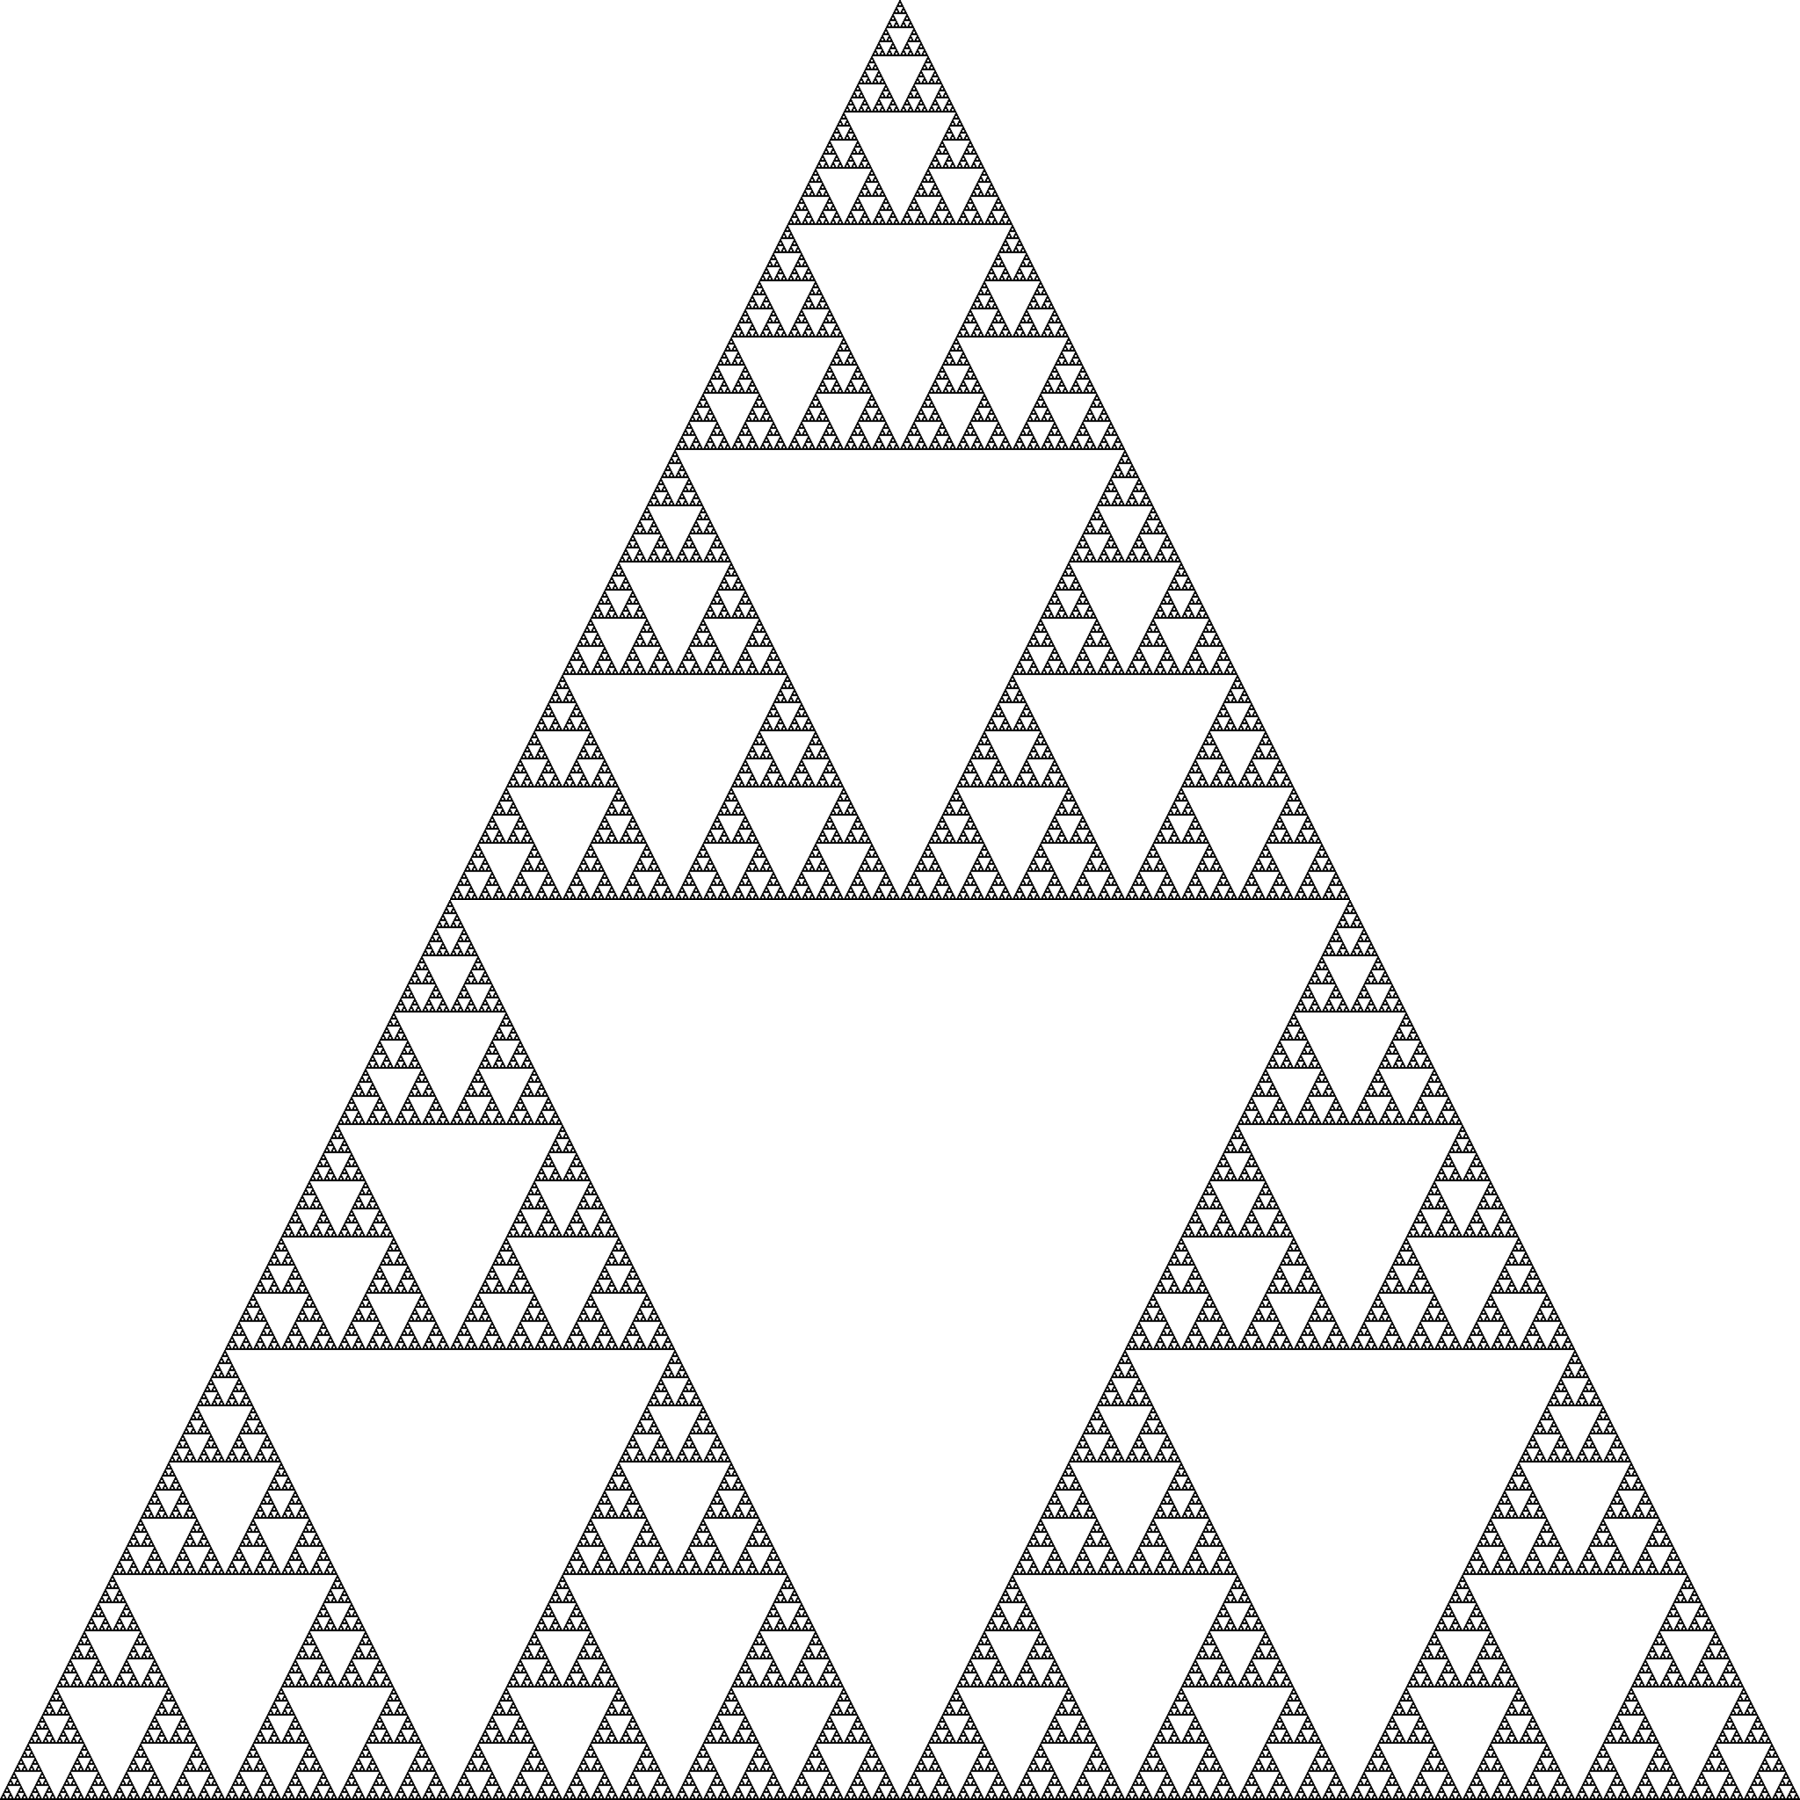
\includegraphics[width=0.5\textwidth]{papers/ifs/images/sierpinski}
	\caption{Sierpinski-Dreieck}
	\label{ifs:sierpinski10}
\end{figure}
Wenn man das Dreieck genau anschaut, erkennt man schnell, dass es aus drei kleineren Kopien seiner selbst besteht.
Es ist also ein Selbstähnliches Konstrukt.
Diese Eigenschaft wollen wir uns zunutze machen.


Wir definieren das Dreieck mit Kantenlänge 1 als Menge $X$.
Ausserdem bestimmen wir drei Funktionen, welche die gesamte Menge auf eine ihrer kleineren Kopien abbildet
\begin{align*}
	f_1(x,y)
	= 
	\begin{pmatrix}
		\frac{1}{2} & 0 \\
		0 & \frac{1}{2} \\
	\end{pmatrix}
	\begin{pmatrix}
		x\\
		y\\
	\end{pmatrix} 
	,\quad
	f_2(x,y)
	= 
	\begin{pmatrix}
		\frac{1}{2} & 0 \\
		0 & \frac{1}{2} \\
	\end{pmatrix}
	\begin{pmatrix}
		x\\
		y\\
	\end{pmatrix} 
	+
	\begin{pmatrix}
		\frac{1}{2} \\
		0
	\end{pmatrix}
	, \quad
	f_3(x,y)
	= 
	\begin{pmatrix}
		\frac{1}{2} & 0 \\
		0 & \frac{1}{2} \\
	\end{pmatrix}
	\begin{pmatrix}
		x\\
		y\\
	\end{pmatrix} 
	+
	\begin{pmatrix}
		\frac{1}{4} \\
		\frac{1}{2}
	\end{pmatrix}\\
\end{align*}
$f_1$ bildet das Dreieck auf das Teilstück unten links ab, $f_2$ auf das Teilstück unten rechts und $f_3$ auf das obere Teilstück.
Wendet man alle drei Funktionen auf das Sierpinski-Dreieck an, entsteht also wieder ein Sierpinski-Dreieck.
\begin{align*}
	X = \bigcup\limits_{i = 1}^{3} f_i(X)
\end{align*}
Man kann sogar noch einen Schritt weiter gehen, und sagen: Wenn wir die Funktionen auf eine beliebige Startmenge anwenden, konvergiert die Menge gegen das Sierpinski-Dreieck.
\begin{figure}	
	\centering
	\subfigure[]{
		\label{ifs:sierpconsta}
		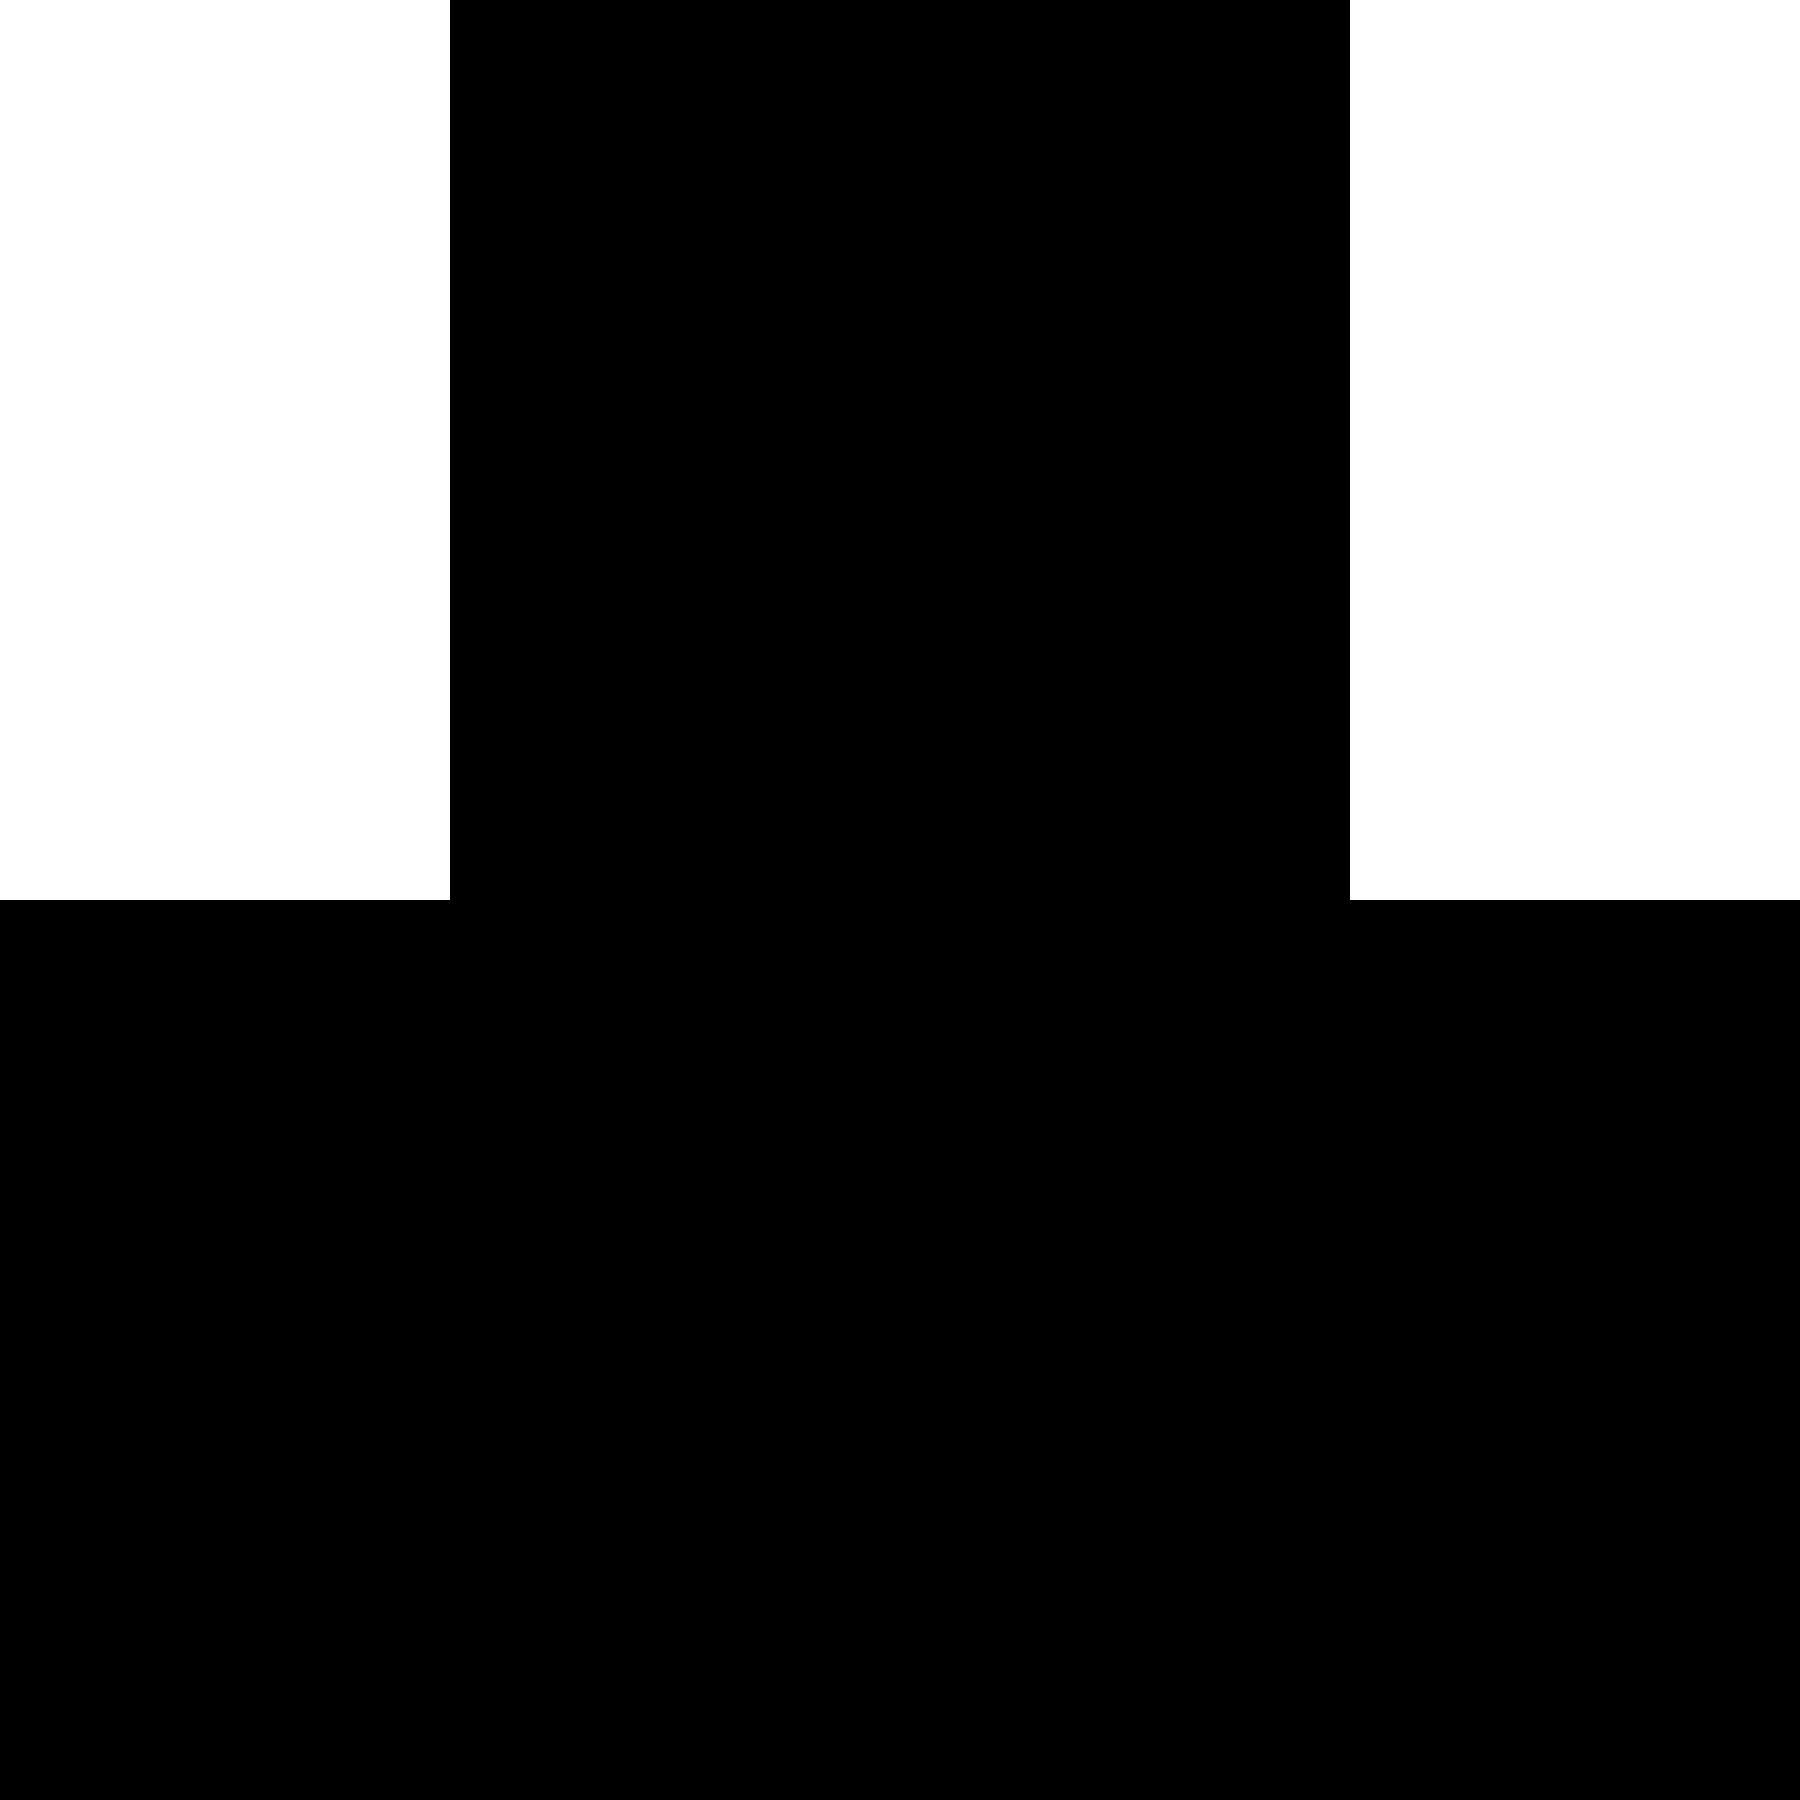
\includegraphics[width=0.25\textwidth]{papers/ifs/images/sierpinski1}}
	\subfigure[]{
		\label{ifs:sierpconstb}
		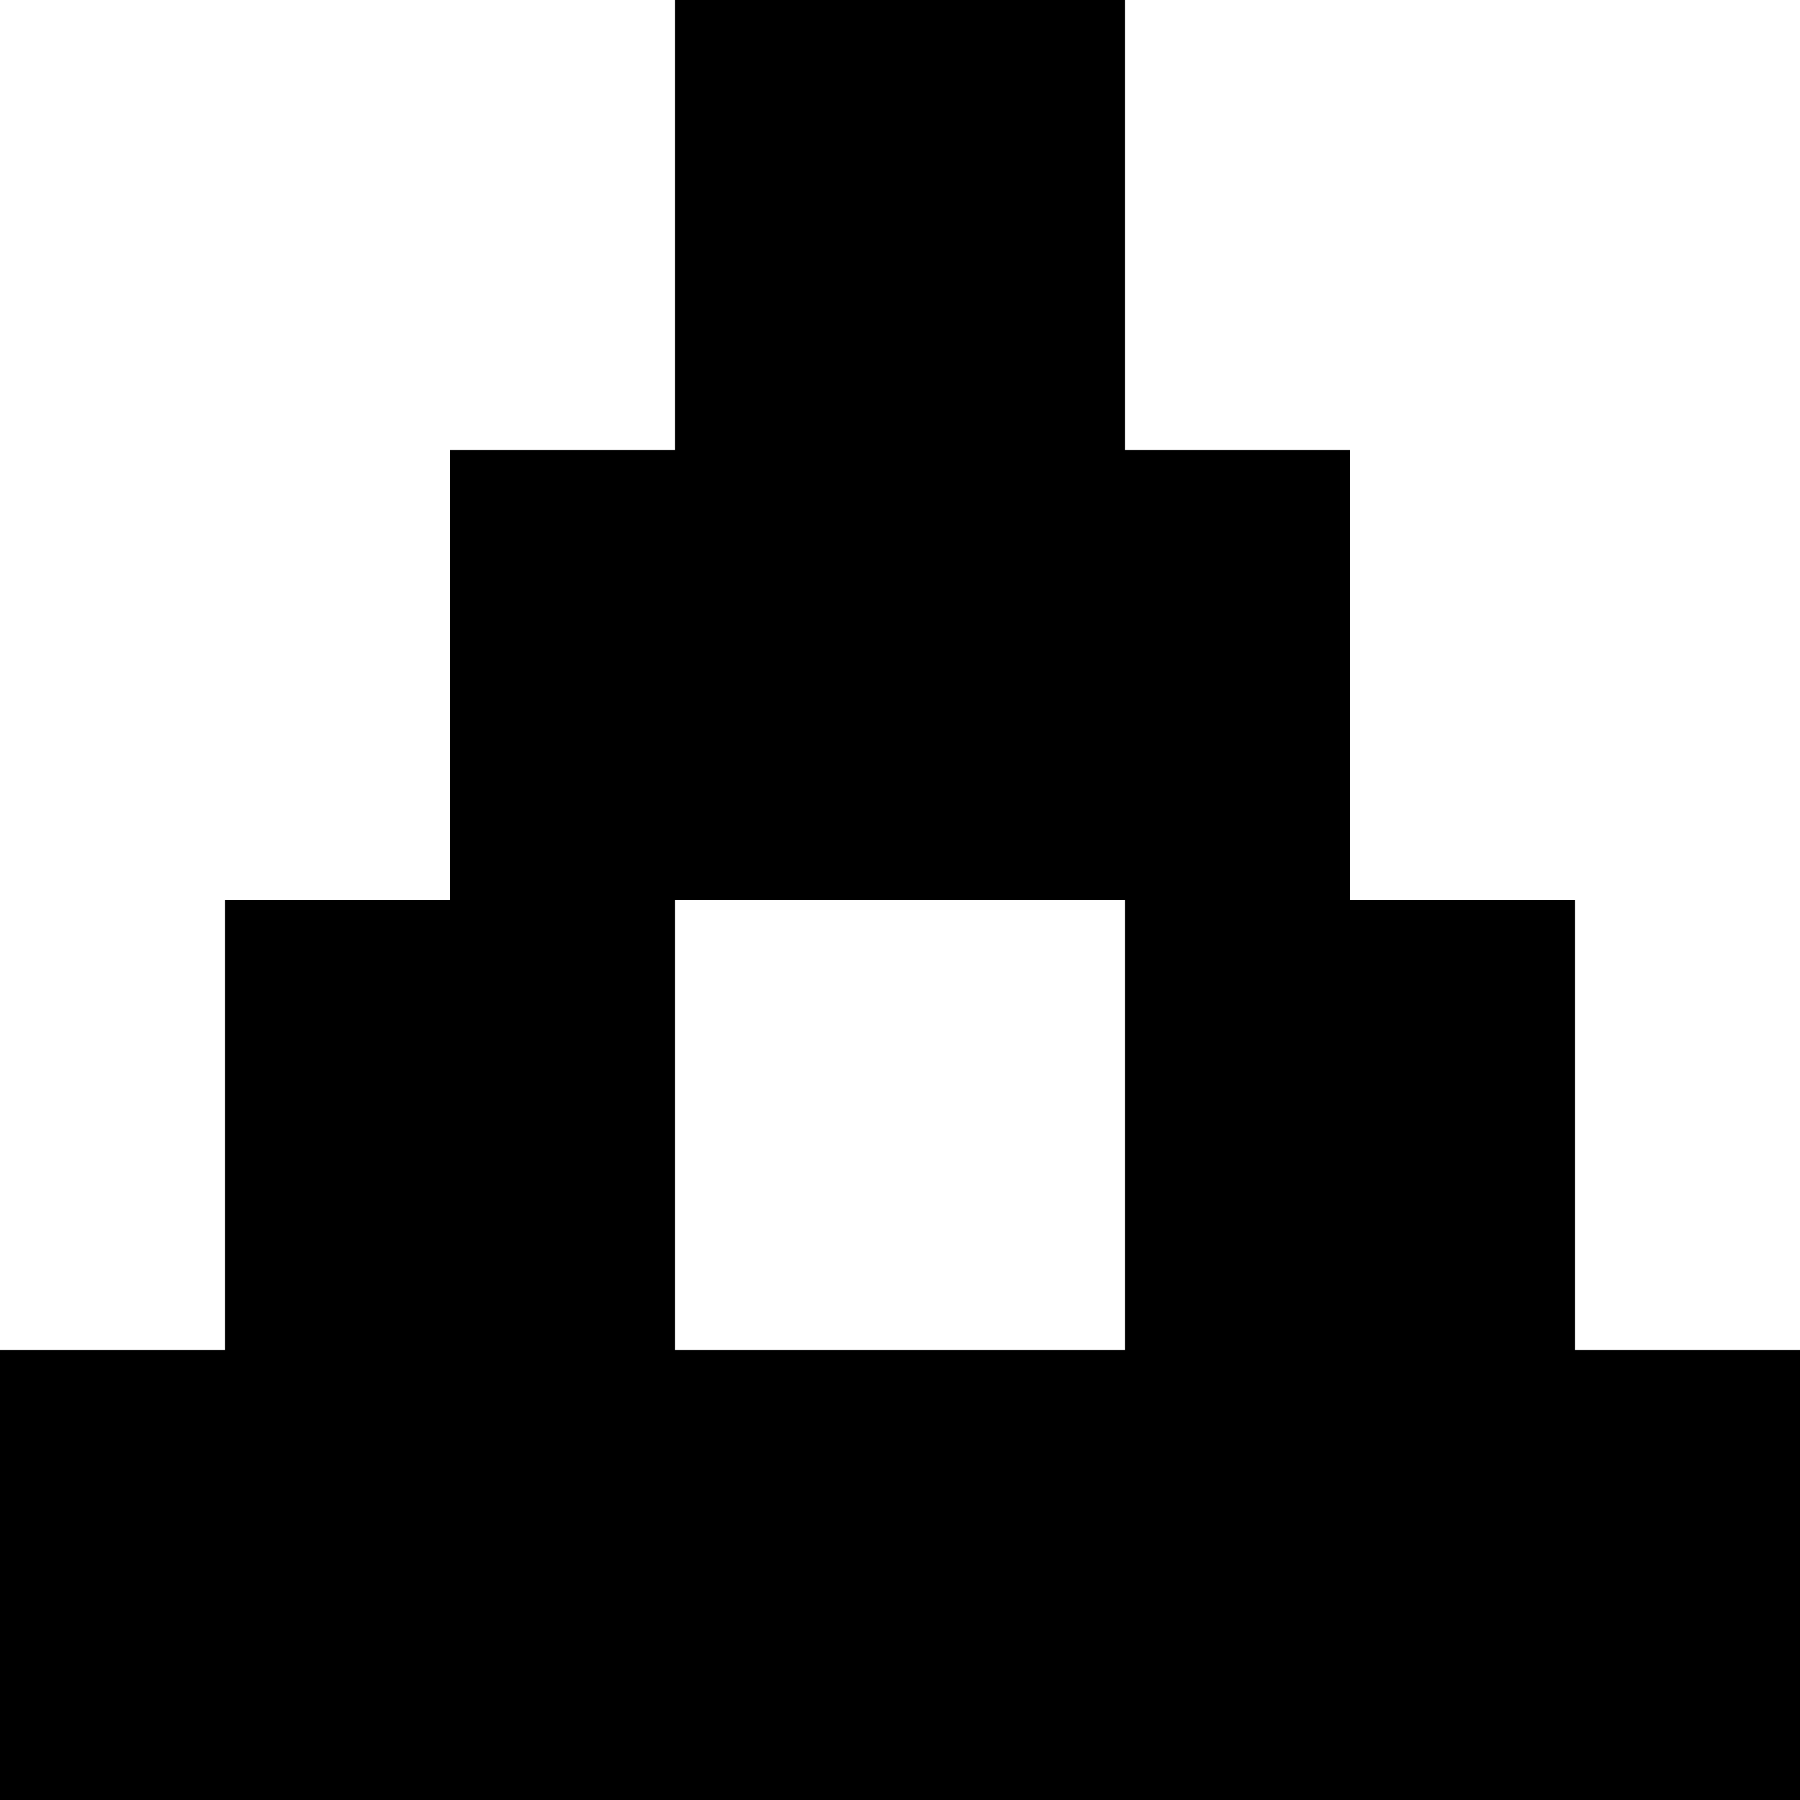
\includegraphics[width=0.25\textwidth]{papers/ifs/images/sierpinski2}} 
	\subfigure[]{
		\label{ifs:sierpconstc}
		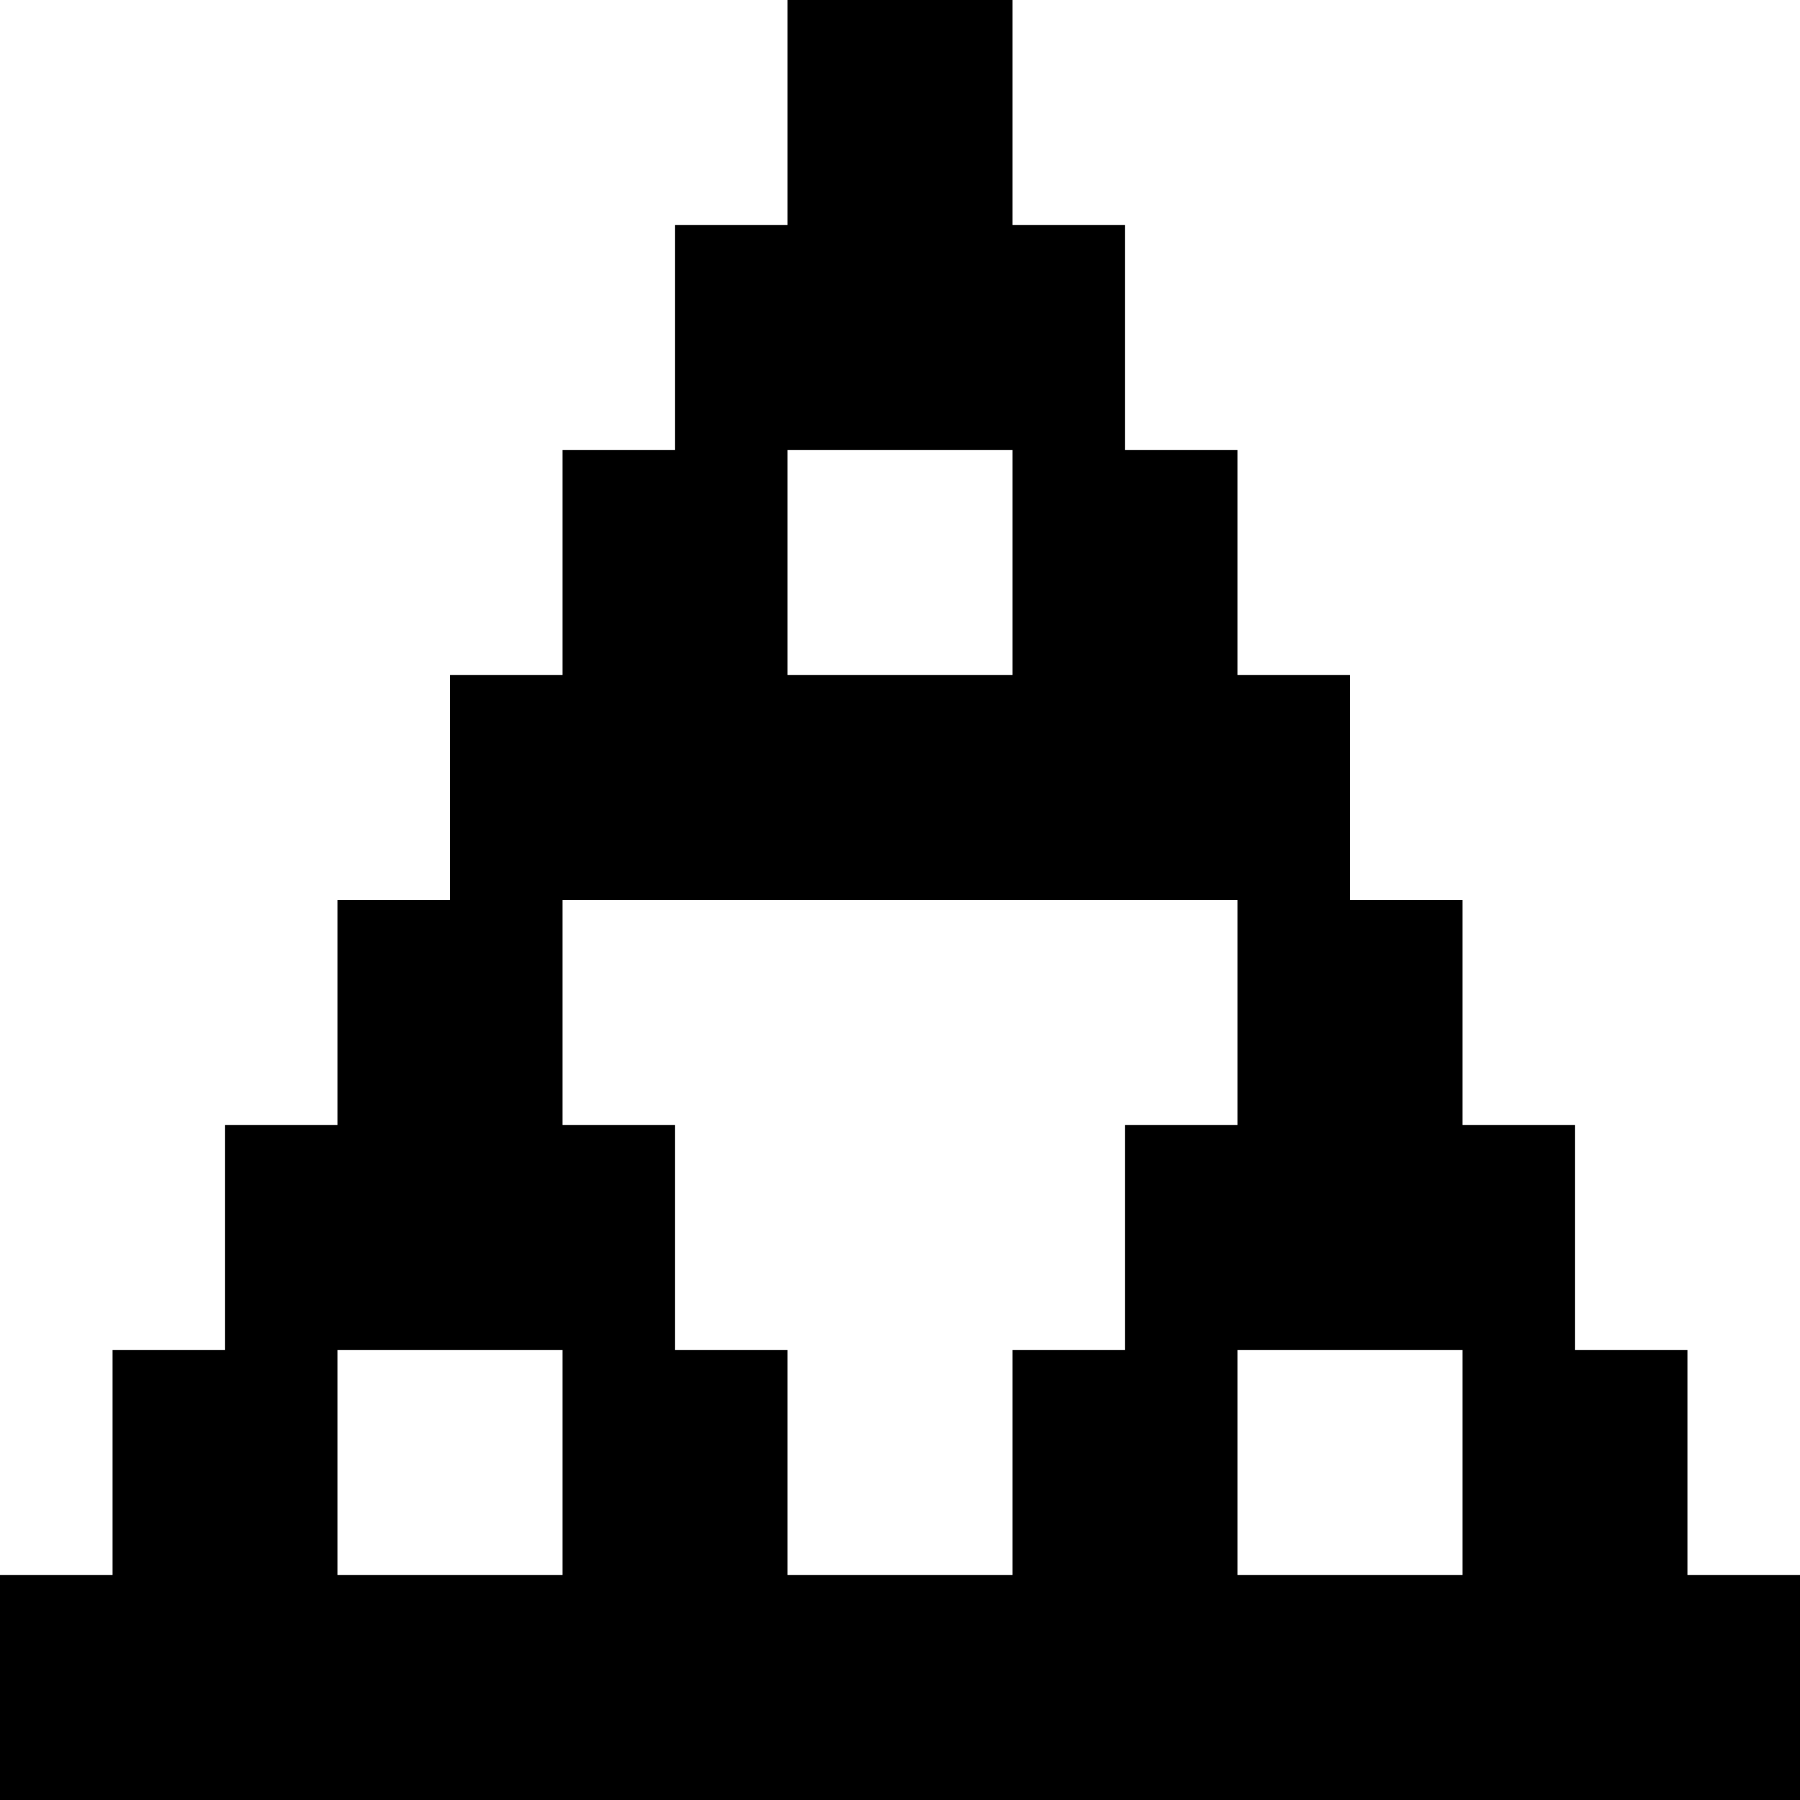
\includegraphics[width=0.25\textwidth]{papers/ifs/images/sierpinski3}}
	\subfigure[]{
		\label{ifs:sierpconstd}
		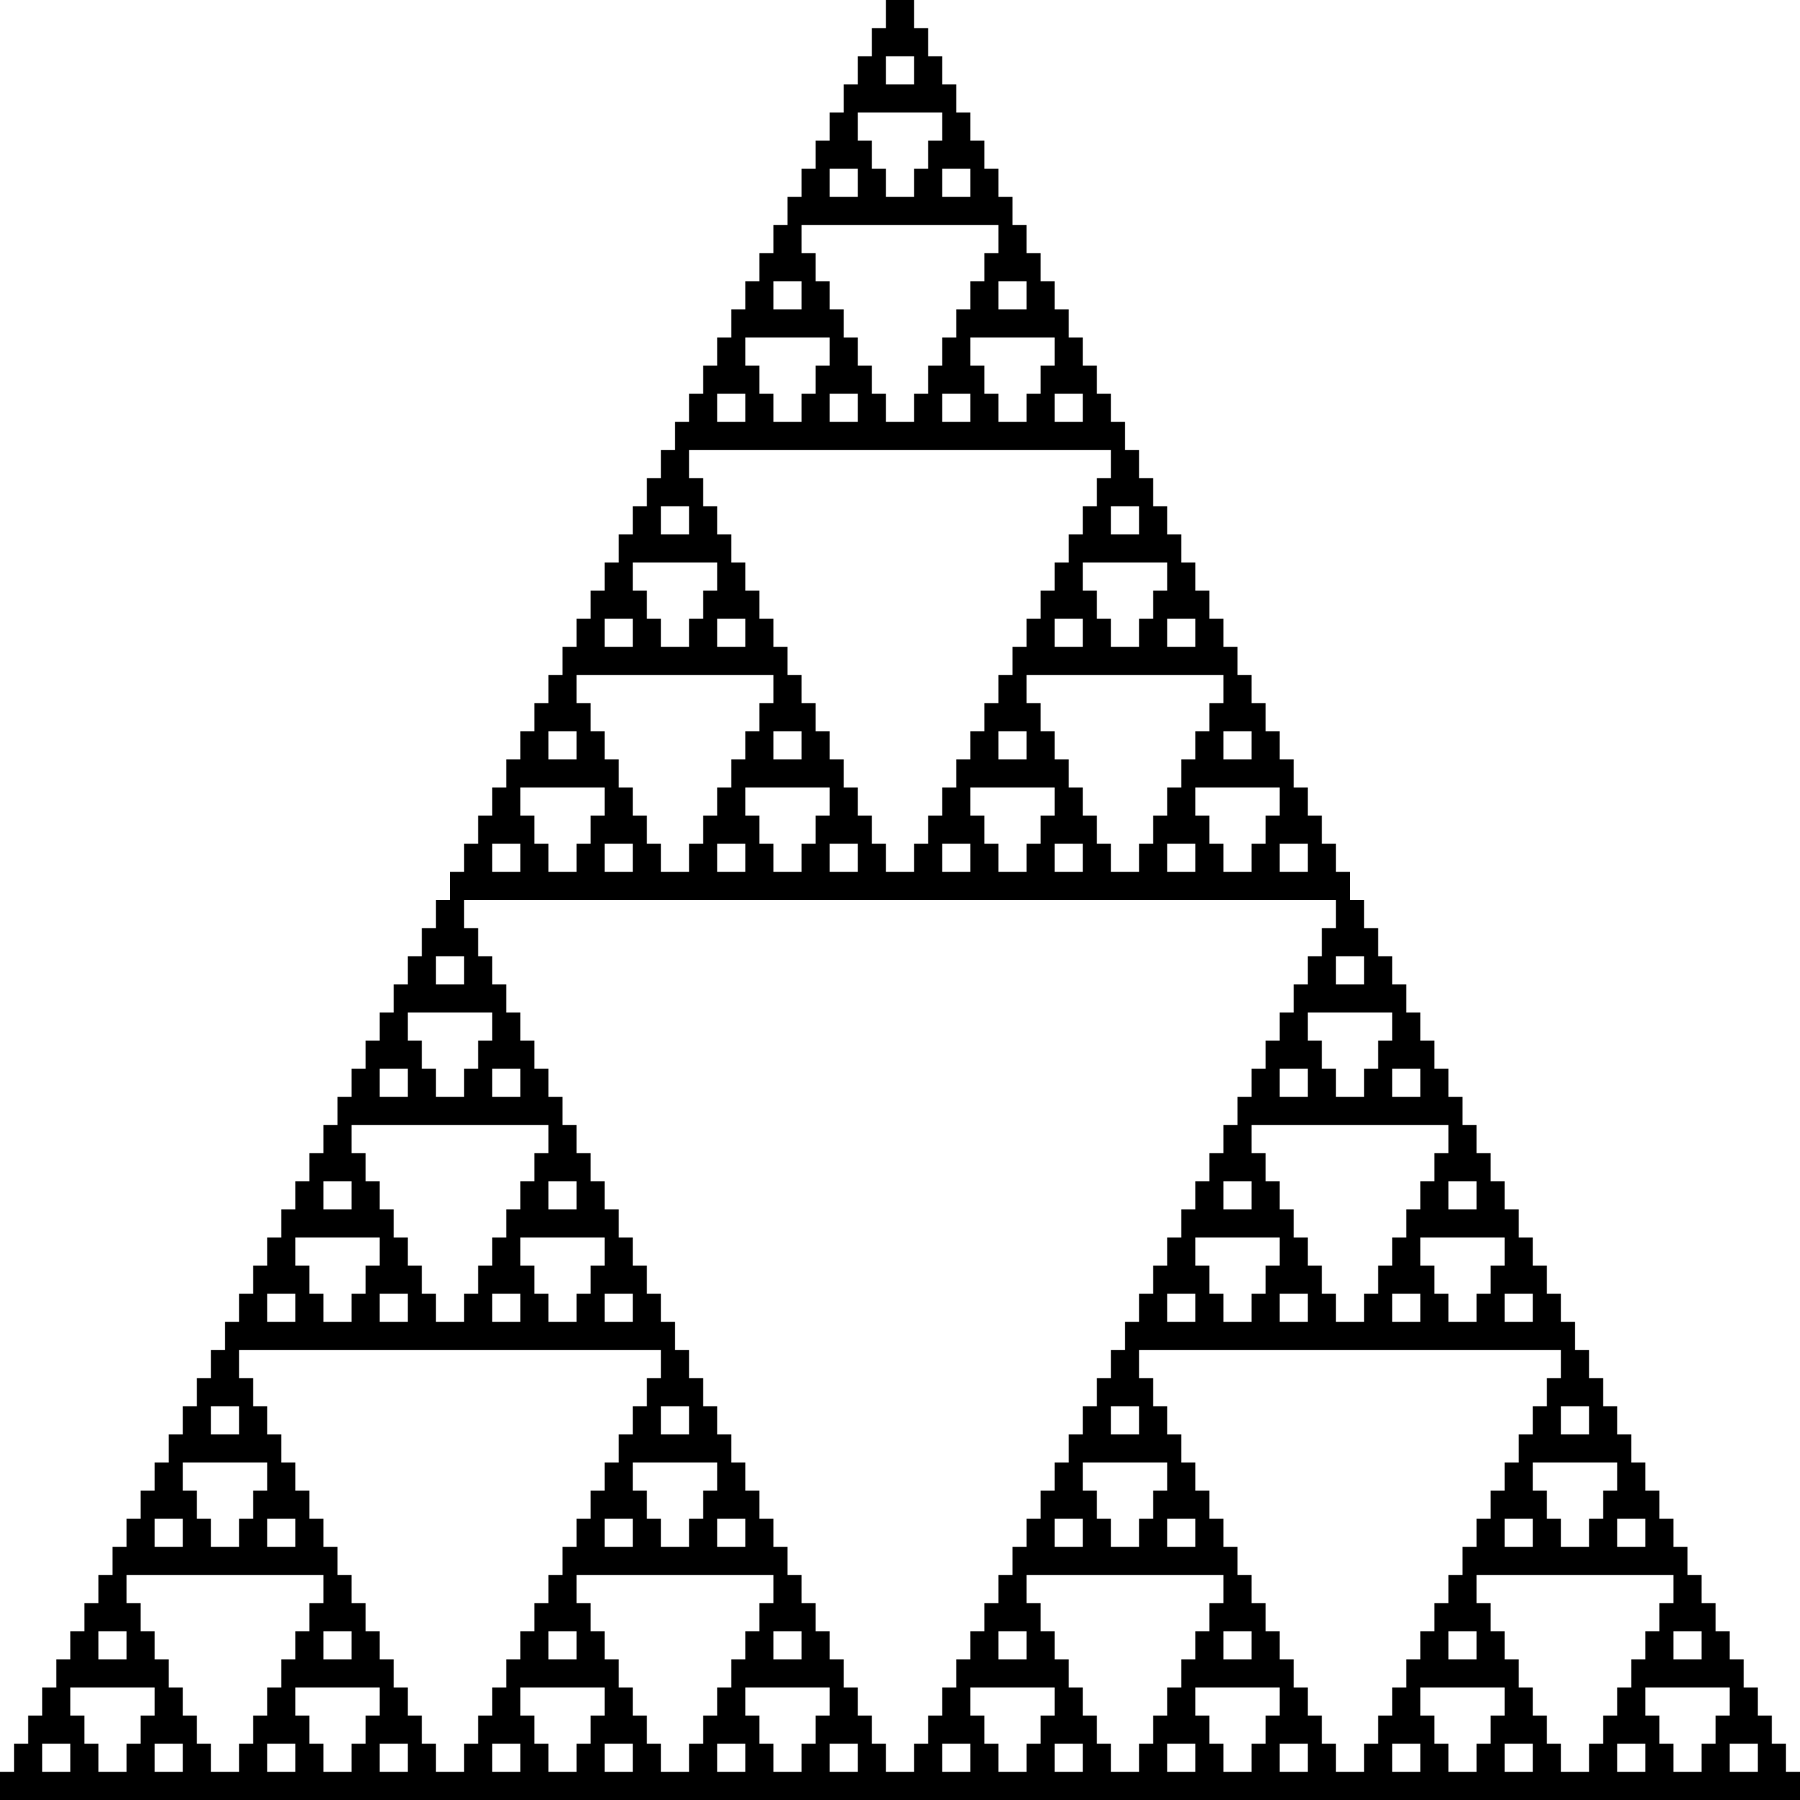
\includegraphics[width=0.25\textwidth]{papers/ifs/images/sierpinski6}}
	\caption{Konstruktion eines Sierpinski-Dreiecks mit einem Schwarzen Quadrat als Start\\
		(a) 1. Iteration (b) 2. Iteration (c) 3. Iteration (d) 5. Iteration}
	\label{ifs:sierpconst}
\end{figure}
Im Beispiel der Abbildung \ref{ifs:sierpconst} sehen wir, wie das Bild nach jeder Iteration dem Sierpinski-Dreieck ähnlicher wird.
Der Abstand zum Original wird immer kleiner, und konvergiert bei unendlich Iterationen gegen null.

\subsection{Iterierte Funktionensysteme
\label{ifs:subsection:bonorum}}
In diesem Unterkapitel wollen wir die Erkenntnis, wie wir aus einer beliebigen Menge ein Sierpinski-Dreieck generieren können, verallgemeinern.


$S_1,...,S_n$ sind Kontraktionen auf die Menge $D \subset \mathbb{R}^n$. Es gilt
\begin{align}
	|S_i(x) - S_i(y)| \leq c_i|x - y|
\end{align}
für jedes i mit einem $c_i < 1$. Dann existiert eine eindeutige kompakte Menge $F$ für die gilt
\begin{equation}
	F = \bigcup\limits_{i = 1}^{m} S_i(F)
\end{equation}
Weiter definieren wir die Transformation S auf kompakte Mengen ohne die leere Menge.
\begin{equation}
	S(E) = \bigcup\limits_{i = 1}^m S_i(E)
\end{equation}
Wird diese Transformation Iterativ ausgeführt, das heisst $S^0(E) = E, S^k(E) = S(S^{k-1}(E))$, und für jedes $i$ $S_i(E) \subset E$, gilt
\begin{equation}
	F = \bigcap\limits_{k = 1}^{\infty} S^k(E).
\end{equation}
In Worte gefasst bedeutet das, dass jede Gruppe von Kontraktionen iterativ ausgeführt, gegen eine eindeutige Menge konvergiert.
Dies für jede Startmenge, solange diese ihre Transformierten wieder beinhaltet.
Auf den Beweis wird verzichtet.
\subsection{Beispiel: Barnsley-Farn}
Der Barnsley-Farn, Abbildung \ref{ifs:farn}, ist ein weiteres Fraktal, welches mit einem IFS generiert werden kann.
Wie man schnell erkennen kann, besteht der Farn aus Blättern, welche eine grosse Ähnlichkeit zum ganzen Farn haben.
\begin{align*}
	{S_1(x,y)}
	= 
	\begin{pmatrix}
		0 & 0 \\
		0 & 0.16 \\
	\end{pmatrix}
	\begin{pmatrix}
		x\\
		y\\
	\end{pmatrix}, \quad
	{S_2(x,y)}
	= 
	\begin{pmatrix}
		0.85 & 0.04 \\
		-0.04 & 0.85 \\
	\end{pmatrix}
	\begin{pmatrix}
		x\\
		y\\
	\end{pmatrix} 
	+
	\begin{pmatrix}
		0 \\
		1.6
	\end{pmatrix}\\
	{S_3(x,y)}
	= 
	\begin{pmatrix}
		0.2 & -0.26 \\
		0.23 & 0.22 \\
	\end{pmatrix}
	\begin{pmatrix}
		x\\
		y\\
	\end{pmatrix} 
	+
	\begin{pmatrix}
		0 \\
		1.6
	\end{pmatrix}, \quad
	{S_4(x,y)}
	= 
	\begin{pmatrix}
		-0.15 & 0.28 \\
		0.26 & 0.24 \\
	\end{pmatrix}
	\begin{pmatrix}
		x\\
		y\\
	\end{pmatrix} 
	+
	\begin{pmatrix}
		0 \\
		0.44
	\end{pmatrix}\\
\end{align*}
In der Abbildung \ref{ifs:farncolor} sehen wir die vier Transformationen farblich dargestellt.

$S_1$ erstellt den Stiel des Farnblattes (rot).
Die Transformation bildet das Gesamte Blatt auf die Y-Achse ab.
$S_2$ (grün) erstellt den Hauptteil des Farnes. 
Sie verkleinert und dreht das gesamte Bild und stellt es auf das Ende des Stiels aus $S_1$.
$S_3$ bildet das gesamte Blatt auf das blaue Teilblatt unten Links ab.
$S_4$ Spiegelt das Blatt und bildet es auf das magentafarbene Teilblatt ab.  

Wir führen im Zusammenhang mit dem Barnsley-Farn \cite{ifs:barnsleyfern} noch eine weitere Methode ein, um IFS auszuführen.
Bis jetzt wurde immer davon gesprochen, die Transformationen auf die gesamte Menge anzuwenden.
Bei komplizierteren IFS welche viele Iterationen brauchen, bis man den Attraktor erkennen kann, ist diese Methode ziemlich rechenintensiv.
Eine Alternative ist das Chaosspiel \cite{ifs:chaos}. 
Bei dieser Methode werden die Transformationen nicht auf die Menge angewendet, sondern nur auf einen einzelnen Punkt.
Der Startpunkt kann dabei ein beliebiger Punkt in $E$ sein.
Es wird bei jedem Iterationsschritt nur eine Transformation, welche zufällig gewählt wurde, angewendet.
Da, wie wir beim Barnsley-Farn gut sehen, dass nicht jede Transformation gleich viel des Bildes ausmacht, werden diese beim Chaosspiel gewichtet.
Die Gewichtung erfolgt über den Anteil der Gesamtmasse.
Im Fall des Barnsley-Fern wird $S_1$ in $1\%$, $S_2$ in $85\%$ und $S_3 \& S_4$ in $7\%$ der Iterationen ausgeführt. 
\begin{figure}	
	\centering
	\makebox[\textwidth][c]{
		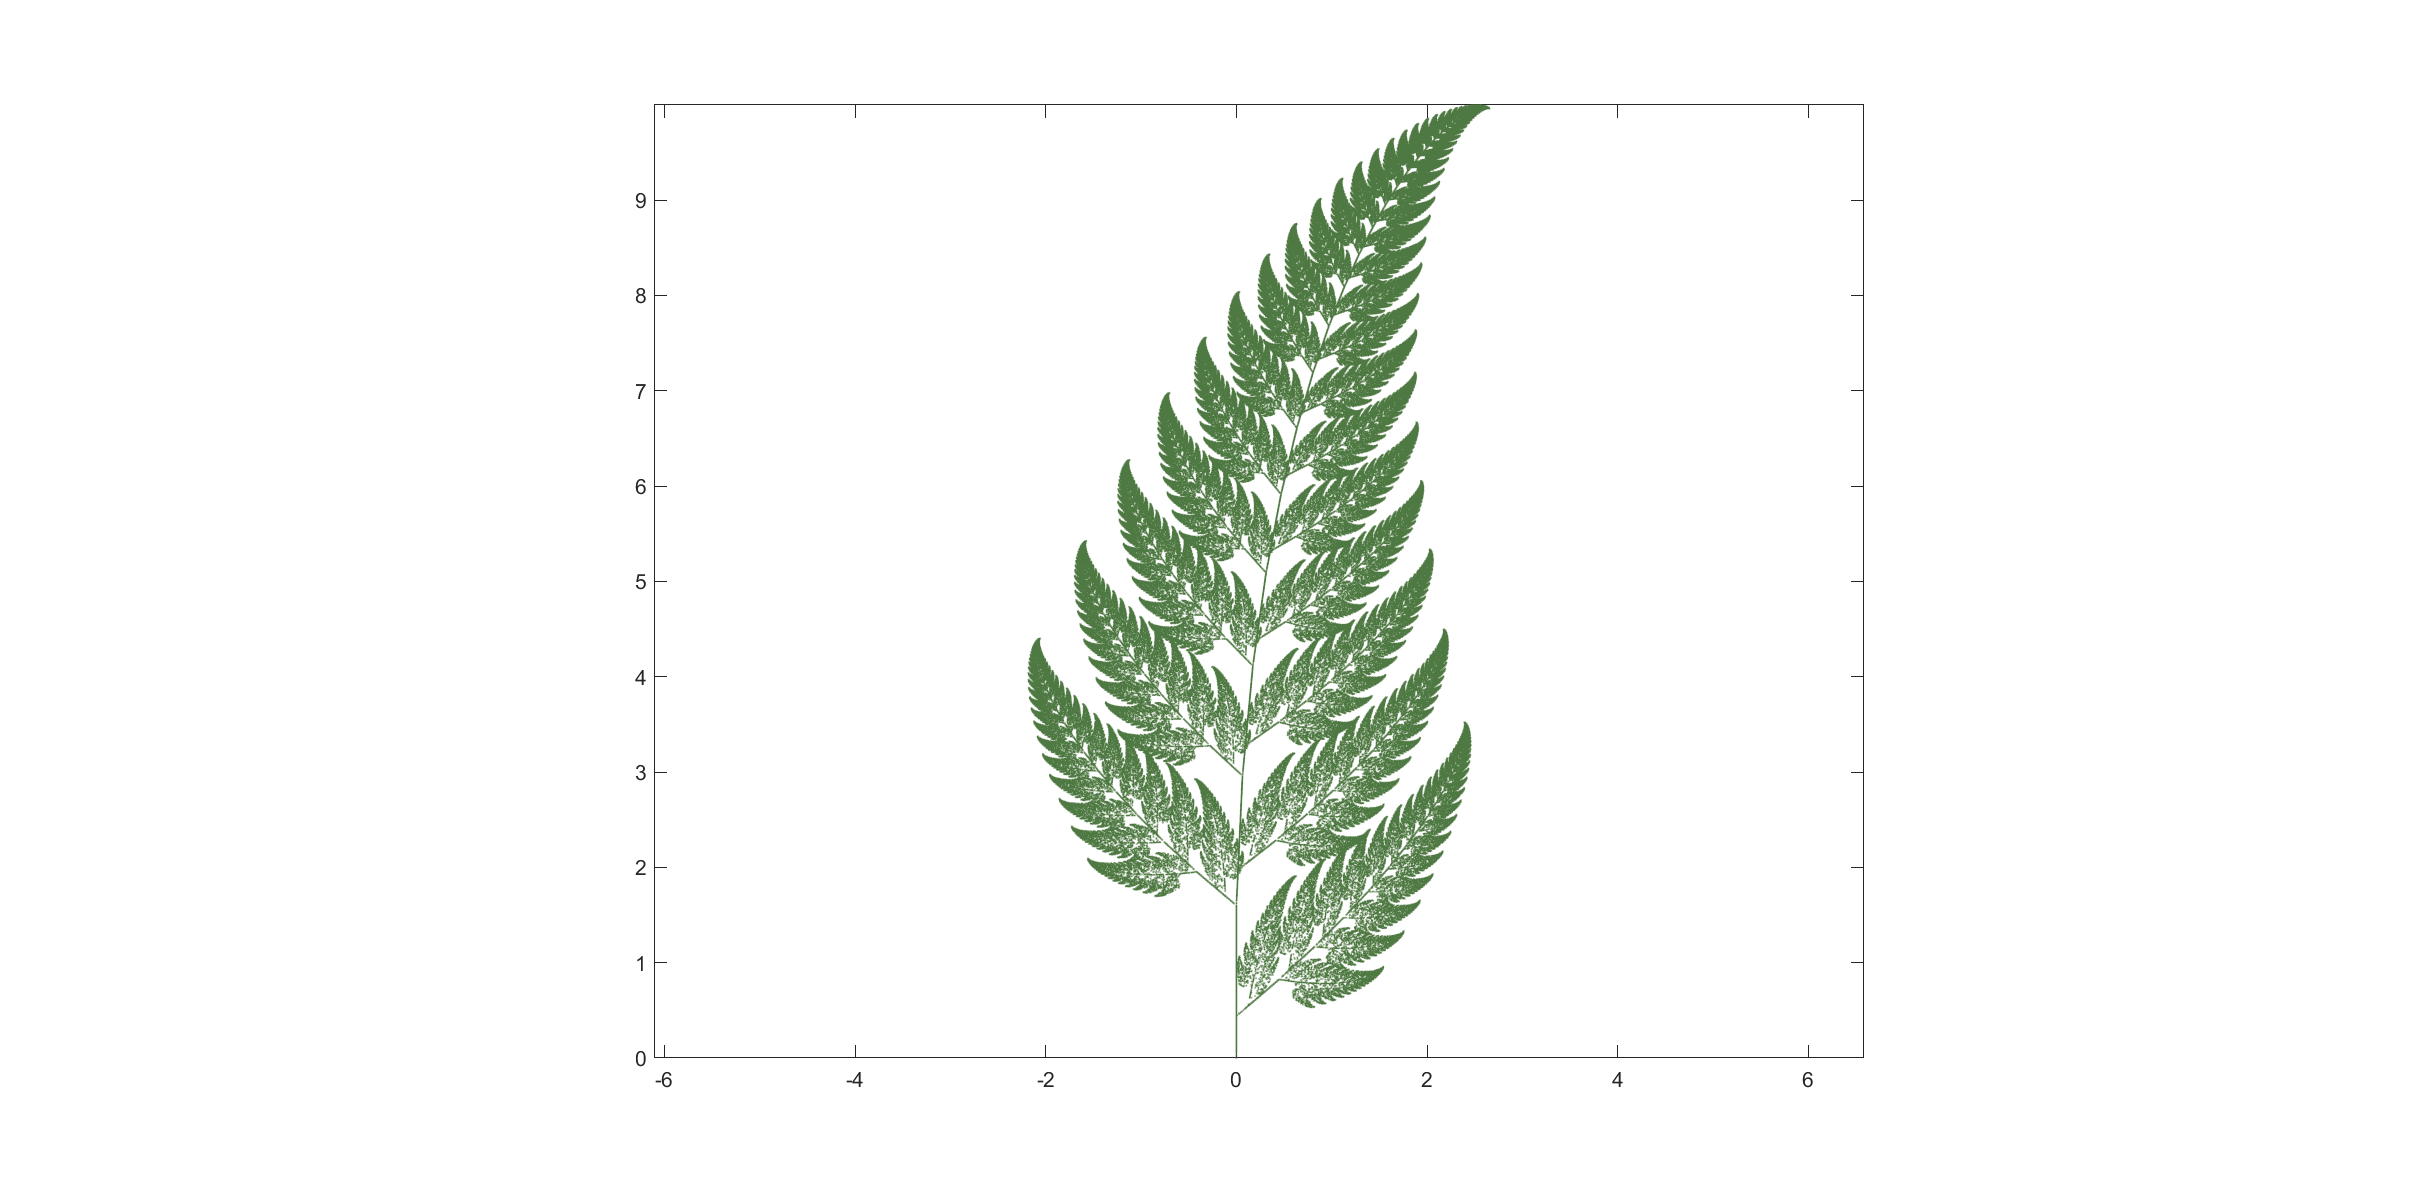
\includegraphics[width=1.4\textwidth]{papers/ifs/images/farn}}
	\caption{Barnsley-Farn}
	\label{ifs:farn}
\end{figure}
\begin{figure}
	\centering
	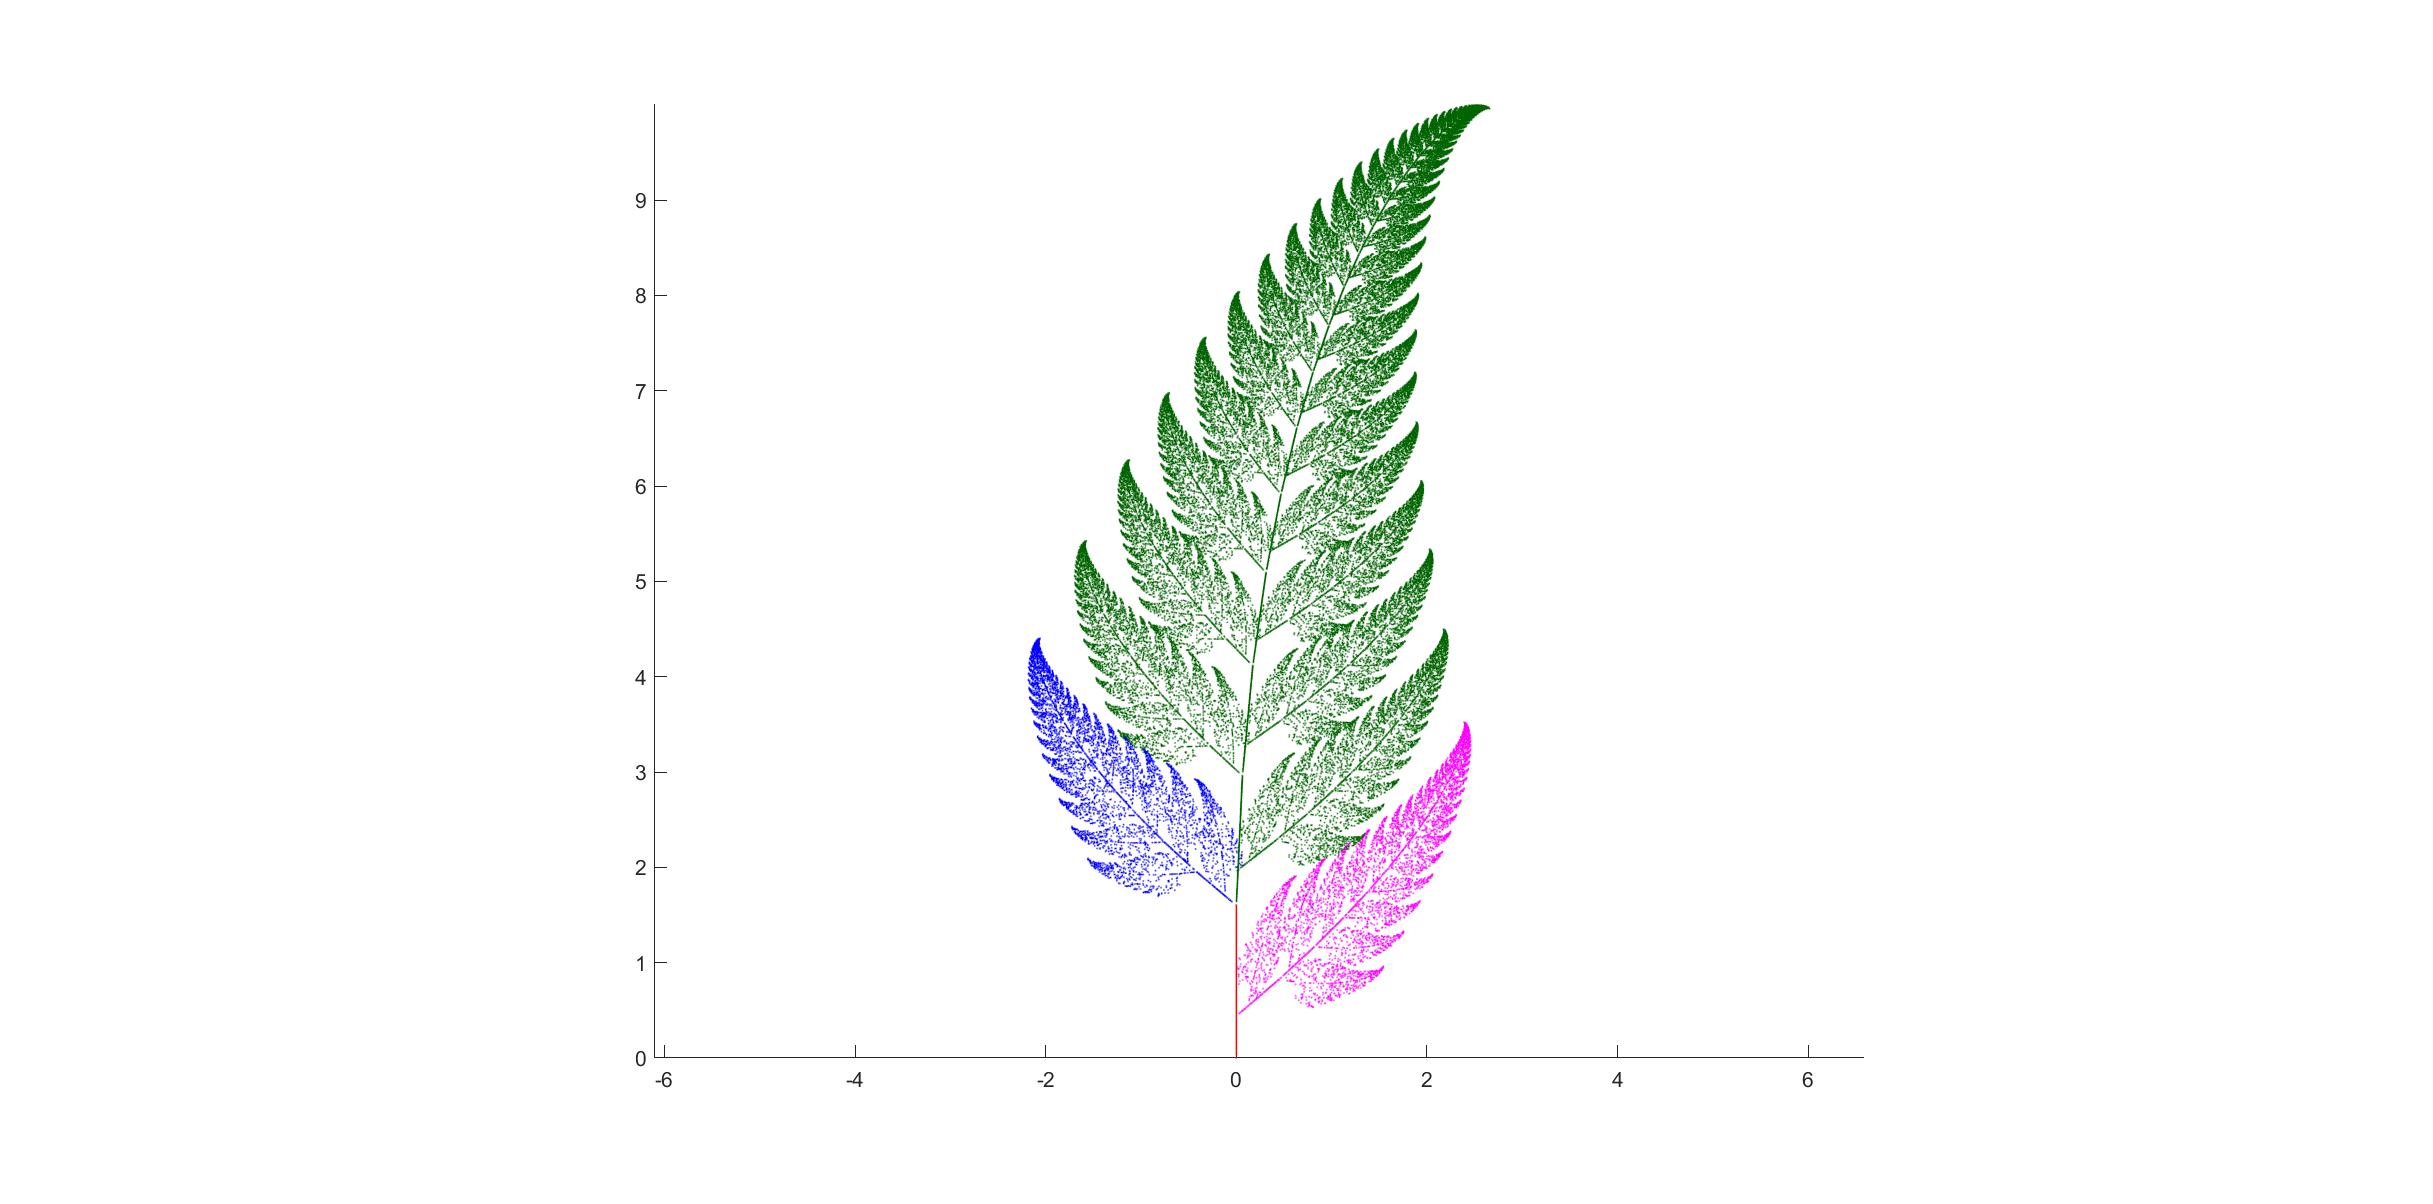
\includegraphics[width=0.7\textwidth]{papers/ifs/images/farncolor}
	\caption{Vier Transformationen des Barnsley-Farn}
	\label{ifs:farncolor}
\end{figure}
